\section{System's Perspective}
\label{ch:sys_persp} % used to ref this chapter

This section covers the main modules of the system with their  
respective technologies and dependencies, as well as how they
were deployed.

\subsection{Module view}

\begin{figure}[H]
    \centering
    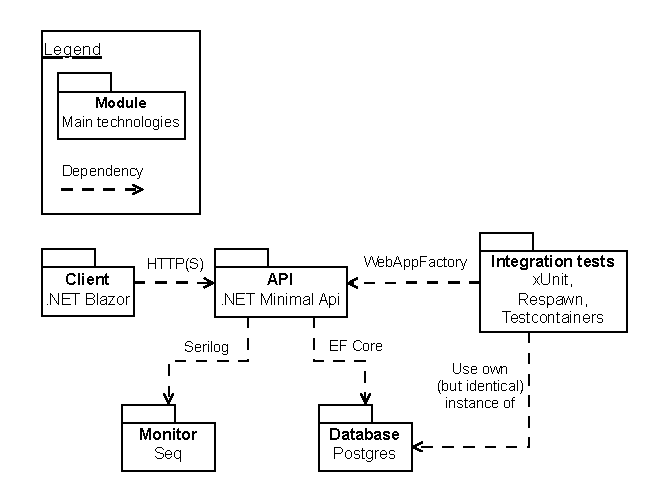
\includegraphics[width=\linewidth]{images/modules.drawio.pdf}
    \caption{Diagram showing the modules that make up the system with
    their dependencies and main technologies.}
    \label{fig:modules}
\end{figure}

Users interact with the system through the Client module,
which send requests to the API module. The API has a database 
connection and writes logs which are read by the Monitor module.
The Integration tests use services from the API and its own instances
of the database to test the API module.
This is illustrated in Figure \ref{fig:modules}.

\subsection{Deployment view}

\begin{figure}[H]
      \centering
      \makebox[\linewidth]{
      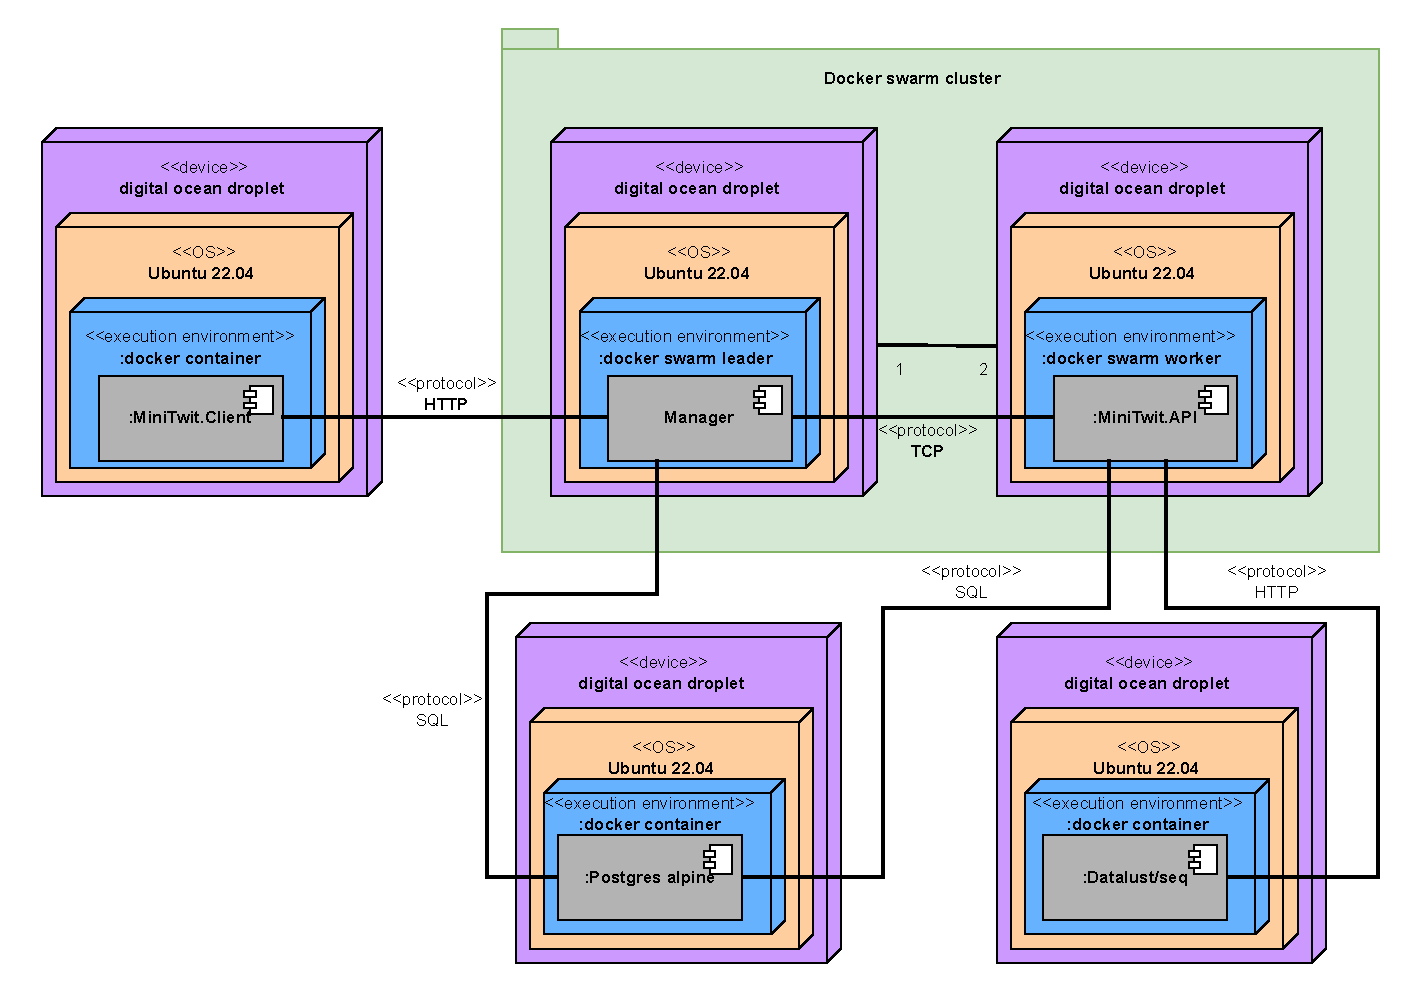
\includegraphics[width=1.4\textwidth]{images/deployment_diagram.drawio.pdf}}
      \caption{Deployment diagram showing how the modules were deployed.}
      \label{fig:deployment_diagram}
\end{figure}

We used Digital Ocean to deploy our system.
The modules were deployed to ``droplets'' running Ubuntu 22.04.
This is illustrated in Figure \ref{fig:deployment_diagram}.
It worked by creating and pushing docker images that the 
droplets pulled and ran.

\subsection{API}

The API functions as a backend for the MiniTwit application.
It is deployed as three separate units. 
It uses docker swarm with one leader/manager 
giving tasks to two workers. Thus, the leader functions as a 
load balancer using the workers as servers.
We decided that the leader should not be a worker,
because we wanted to function optimally as a load balancer.
We were not sure, how it would be affected by being another worker.
Instead we can use it to run other side tasks, like databse migrations.

The API project is implemented in .NET using minimal API.
The database communication is done using Entity Framework Core.
It logs using Serilog\cite{serilog}, 
which is configured to write to Seq\cite{seq}.

\subsection{Client}

The Client is the frontend for the MiniTwit application.
It is implemented as a Blazor webassembly app.
This means the load is distributed to the users' browsers 
rather than a server.
It sends requests to and receives responses from the API module.

\subsection{Monitor}

Our Monitor uses the tool, Seq\cite{seq}.
It handles logs and displays custom graphs based on 
the log information. We have both developer relevant 
graphs such as API response times and errors,
as well as business relevant graphs such as number 
of newly registered users and messages posted.
It is deployed on its own Digital Ocean droplet 
using an image provided by datalust\cite{seq}.

\subsection{Database}

The database is a PostgreSQL\cite{postgres} database.
It contains information about registered users,
posted messages, and followers.

\subsection{Sequence diagram}

\begin{figure}[H]
    \centering
    \makebox[\linewidth]{
    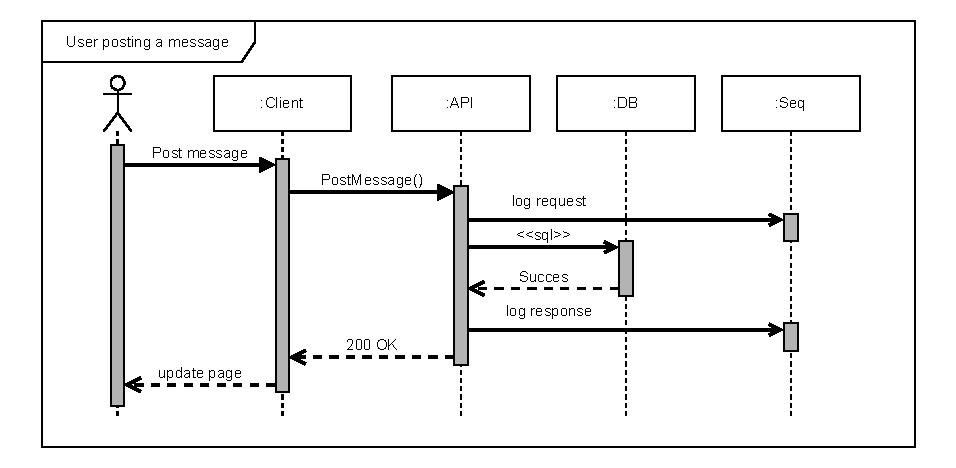
\includegraphics[width=1.4\textwidth]{images/sequence_diagram.drawio.pdf}}
    \caption{Sequence diagram showing how the system acts upon 
    a user successfully posting a message.}
    \label{fig:seq_diagram}
\end{figure}

In summary, users post messages from the Client.
The Client sends requests to the API, which logs the request 
information, saves the messages to the database, 
logs the reponse information and sends responses back to the 
Client. Logs are used for monitoring in Seq. 
The Client then updates the UI for the users.
This is illustrated in Figure \ref{fig:seq_diagram}.
